In diesen Kapitel wird die Problemstellung der Reparatur und die im Paper als
state-of-the-art bekannten Reparaturmethoden vorgestellt.  Die Reparatur mit
der Anomalienerkennung ARX wird im zweiten Kapitel wichtig, da die im Paper als
neue Methodik vorgestelltes IMR iterativ auf ARX aufbaut.  Die Stellvertreter
der anderen Methoden werden zusätzlich bei der Evaluierung von IMR zum
Vergleich herangezogen.

\subsection{Problemstellung der Reparatur}

Es sei $x = x[1],\dots,x[n]$ eine Zeitreihe, die aus einer Messung erhoben
wurde und tendenziell unkorrekte Werte enthalten kann. Kurz wird ein
Datenpunkt $x[i]$ mit $x_i$ für jeden Zeitpunkt $i \in
\{1,2,\dots,n\}$ bezeichnet. Zudem sei $x^{\text{truth}}$ dieselbe Zeitreihe
mit unvollständigen, aber dafür absolut korrekten (markierten) Werten.
\[
    x^{\text{truth}}_i = \left\{
\begin{array}{ll}
    x^{\text{truth}}_i = w_i&, \text{falls ein korrekter Datenpunkt }w_i
    \text{ für den Zeitpunkt }\\
&~ i \text{ bekannt ist.}\\
    \text{\_\_}&, \text{ansonsten}
\end{array}
 \right.
\]
Neben diesen beiden Zeitreihen sei $x^{\text{truth*}}$ die vollständig bekannte
und absolut korrekte Zeitreihe. Gesucht ist ein Verfahren, das für eine beliebige
Zeitreihe $x$ und ein zugehöriges $x^{\text{truth}}$ eine reparierte Zeitreihe
$y$ ohne der Kenntnis von $x^{\text{truth*}}$ ermittelt, sodass die Abweichung von y
zu $x^{\text{truth*}}$ minimal ausfällt. Jeder bekannte Wert von
$x^{\text{truth}}$ ist dann in $y$ enthalten. Lediglich Werte in y, die in
$x^{\text{truth}}$ unbekannt bzw.\ auf \_\_ gesetzt sind, sind die reparierten
Werte von $x$.
\\
\\
Eine Abweichung ist hierbei minimal, wenn der RMS-Fehler $\Delta$ minimal ist:
\[
    \Delta\left(x^{\text{truth*}}, y\right) = \sqrt{\frac{1}{n} \sum_{i=1}^n \left( x^{\text{truth*}}_i - y_i \right)^2}
\]
~\\
\\
\textbf{Beispiel 1}. Es seien folgende Zeitreihen $x$, $x^{\text{truth}}$, $x^{\text{truth*}}$ und eine Reparatur $y$ gegeben:
\begin{itemize}
    \item $x =                 \{6, 10, 9.6, 8.3, 7.7, 5.4, 5.6, 5.9, 6.3, 6.8, 7.5, 8.5\}$
    \item $x^{\text{truth}} =  \{6, 5.6, 5.4,  \_\_, \_\_,5.4, \_\_,\_\_,\_\_,\_\_,\_\_,8.5\}$
    \item $x^{\text{truth*}} =  \{6, 5.6, 5.4,  5.2, 5.3, 5.4, 5.6, 5.9, 6.3, 6.8, 7.5, 8.5\}$
    \item $y =  \{6, 5.6, 5.4,  5.2, 5.4, 5.4, 5.6, 5.9, 6.3, 6.8, 7.5, 8.5\}$
\end{itemize}
\begin{figure}
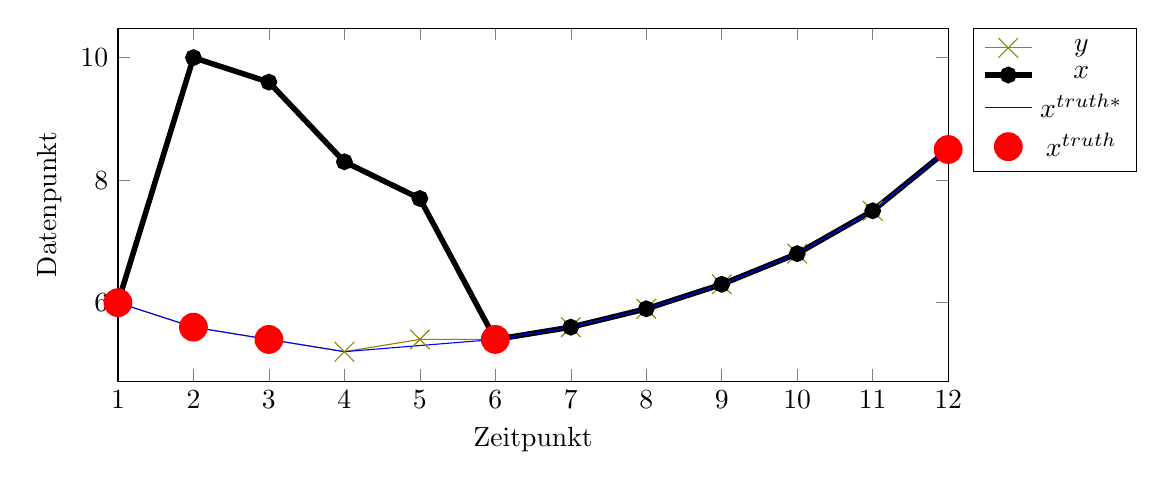
\begin{tikzpicture}
\begin{axis}[width=\textwidth,
    height=.5\textwidth,
xlabel=Zeitpunkt,
ylabel=Datenpunkt,
legend pos=outer north east,
xmin=1,
xmax=12
]
\addplot[olive,mark size=5.0pt, mark=x] table{
Zeitpunkt Wert 
1 6
2 5.6
3 5.4
4 5.2
5 5.4
6 5.4
7 5.6
8 5.9
9 6.3
10 6.8
11 7.5
12 8.5
};
\addlegendentry{$y$}
\addplot[black, line width=2.0pt, mark size=2.0pt, mark=*]  table{
Zeitpunkt Wert 
1 6
2 10
3 9.6
4 8.3
5 7.7
6 5.4
7 5.6
8 5.9
9 6.3
10 6.8
11 7.5
12 8.5
};
 \addlegendentry{$x$}
    \addplot[blue,mark size=5.0pt] table{
Zeitpunkt Wert 
1 6
2 5.6
3 5.4
4 5.2
5 5.3
6 5.4
7 5.6
8 5.9
9 6.3
10 6.8
11 7.5
12 8.5
};
\addlegendentry{$x^{\text{truth*}}$}
\addplot[only marks, red, mark size=5.0pt] table{
Zeitpunkt Wert 
1 6
2 5.6
3 5.4
6 5.4
12 8.5
};
\addlegendentry{$x^{\text{truth}}$}
% if you have the file, you can do
% \addplot table {datafile.csv};
\end{axis}
\end{tikzpicture}
    \caption{Beispiel 1.}\label{fig:1}
\end{figure}
~\\
In der Abb.\ \ref{fig:1} sind die Zeitreihen eingetragen. Es lässt sich
erkennen, dass Messfehler bei den Zeitpunkten 2 bis 5 durch eine nach oben
angeordnete Verschiebung der Werte auftreten.  Zudem lassen sich zwei Vorteile
von markierten Werten $y^{\text{truth}}$ erkennen.  Einerseits können die Werte
direkt in die Reparatur $y$ einfliessen, andererseits kann durch die
Ermittelung der Abweichungen zu den Messungen geschlussfolgert werden, dass die
umliegenden Zeitpunkte einen ähnlichen oder keinen Fehler aufweisen.  Letzteres
wird ebenfalls von ARX und das darauf aufbauende IMR ausgenutzt (siehe Kapitel
\ref{sec:anomalienerkennung} und \ref{sec:IMR}). In der Darstellung stimmen die
Messungen bei 6 und 12 mit den markierten Werten überein, sodass die Annahme
gemacht werden kann, dass die Messungen 7 bis 11 mit hoher Wahrscheinlichkeit
ebenfalls korrekt sind.  Aufgrund von den zu beobachtenden absteigenden großen
Fehler von Zeipunkt 2 bis 3 lässt sich die Vermutung aufstellen, dass die
Zeitpunkte 4 und 5 ebenfalls absteigend fehlerbehaftet sind. Die Reparatur $y$,
welcher mithilfe des Verfahrens IMR bestimmt wurde, setzt diese Vermutungen um.
In der Darstellung kann lediglich ein geringer Fehler der Reparatur $y$ bei
Zeitpunkt 5 festgestellt werden. Der RMS-Fehler $\Delta$ liegt hier bei $0.03$.   

\subsection{State-of-the-art Repariermethoden}
\subsubsection{Reparatur mit Anomalienerkennung}\label{sec:anomalienerkennung}
    \begin{itemize}
        \item Was ist Reparatur mit Anomalienerkennung (siehe 1.1, 1.2, 7.1 im Paper) 
        \item AR und ARX (siehe 2.2 und 2.3); ARX wird wichtig für IMR, da darauf basierend.
    \end{itemize}
\subsubsection{Bedingungsbasierte Reparatur}

    \begin{itemize}
        \item Was ist Bedingungsbasierte Reparatur (siehe 7.3)
        \item SCREEN (vgl.\ referenzierte Papers) 
    \end{itemize}

\subsubsection{Glättungsbasierte Reparatur}

    \begin{itemize}
        \item Was ist Glättungsbasierte Reparatur (siehe 7.2)
        \item EWMA (vgl.\ referenzierte Papers) 
    \end{itemize}

